%!TEX root = finalReport.tex
%!TEX encoding = UTF-8 Unicode
%==============================================================================

\section{Design Characteristics}
In the following section, the main design characteristics and modeling issues are discussed in order to show how the proposed design procedure can be implemented. It is worth mentioning also that other design characteristics exist and additional features can be considered for specific applications. Thus, the most remarkable design characteristics have been considered as examples for filling in the data in the cause and effect matrix.

\subsection{Robot Body Architecture}
There are two basic architectures of hexapod robots: rectangular and hexagonal as shown in \ref {figure a.png}. The first one has six legs distributed symmetrically along two sides,each side having three legs. The second haslegs distributed axi-symmetrically around the body, in a hexagonal or circular shape.

\begin{figure}[h]
	\centering
	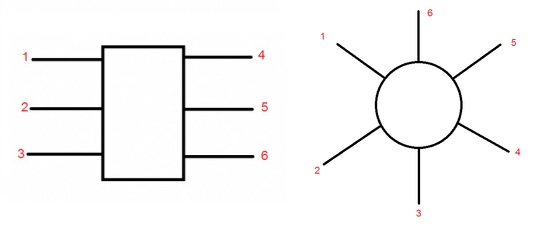
\includegraphics{figure_a}
	\caption{Basic architectures of hexapod robots}
	\label{figure a.png}
\end{figure}

Many references can be found in the literature on rectangular six-legged robots, they describe the longitudinal stability margin for rectangular hexapods. Also, the feasible walking gaits have been widely investigated and tested. Bilateral symmetry may be better suited than radial symmetry to move along a straight line. Rectangular architectures require a special gait for turning action; generally, they need four steps in order to realize a turning action. Hexagonal hexapod robots demonstrate better performances than rectangular robots for some aspects. As example hexagonal robots can have many kinds of gaits and can easily change direction—in fact true radial symmetry implies that all legs are equal and the body has no “front” or “rear”—there is thus no preferential directionfor the motion. It is proved that hexagonal hexapods can easily steerin all directions and that they have a longer stability margin. It isfound that hexagonal robots rotate and move in all directions at the same time,better than rectangular ones, by comparing stability margin and stroke in wave gait.It is proved theoretically that hexagonal hexapod robots have superior stability margin,stride and turning ability compared to rectangular robots.

\subsection{Kinematic Architectures of Legs}
Kinematics architecture depends on the factors related to the application in which the hexapod robot is required for, as for example the terrain form, the workspace and the payload. Literature shows that there is a number of different leg types currently employed for hexapod walking robots. All have advantages and disadvantages. \ref{figure b.png} shows a schematic classification of hexapod legs types.

\begin{figure}[h]
	\centering
	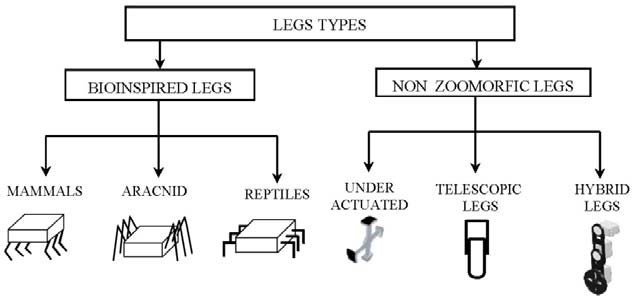
\includegraphics[width =0.8\textwidth]{figure_b}
	\caption{Classification of hexapod legs types}
	\label{figure b.png}

\end{figure}

At the first stage, one can choose between bio inspired and non-zoomorphic legs. Bio inspired leg configuration is motivated primarily by animal gait, such as reptiles, mammals or arachnid. The first one has legs and bodies for moving over rough and uneven terrains. The principal characteristic of the Reptilian type is that the legs are placed on both ends of the protruding body and knees to the side of the base. Mammals’ bodies are above the legs, which gives less support to the base and lower power consumption is needed to support the body, but it requires more stability than other types of animal. In Arachnid configuration, legs extremities are situated on both sides, sticking the knees at the top of the spider’s body. The orientation of the legs in respect to the body of the hexapod robot can be done with three configurations: frontal, sagittal or circular as shown in \ref{figure c.png} .

\begin{figure}[h]
	\centering
	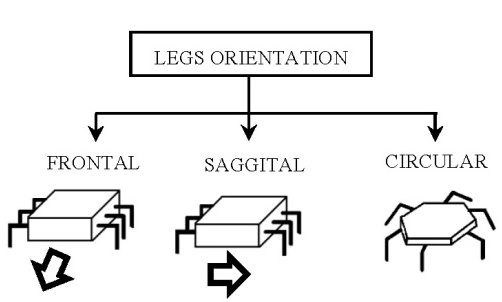
\includegraphics[width =0.8\textwidth]{figure_c}
	\caption{Hexapod leg configurations}
	\label{figure c.png}
\end{figure}

In the first one, the directions are perpendicular to the advancement of the legs’ position, unlike the sagittal, which moves parallel to the robot legs, while in the circular arrangement the legs are positioned radially to the body of the system allowing the mechanism to move in any direction. In the mammalian configuration, the legs are below the body and can place the knees in different positions depending on the application it requires, shown in figure (d). Non zoomorphic legs can be hybrids, telescopic or under-actuated, a solution named Roller-Walker is presented. The principle through which the robot propels itself during wheeled locomotion is the same as that of the skaters.

\begin{figure}[h]
	\centering
	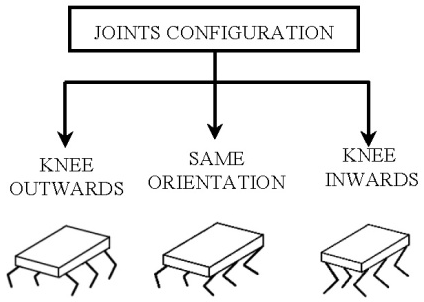
\includegraphics[width =0.8\textwidth]{figure_d}
	\caption{Joint configurations}
	\label{figure d.png}
\end{figure}

\subsection{Actuator Types}
Many kinds of actuators can be employed for operating hexapod walking robots. The majority of hexapods is actuated by electric rotating motors (Servo motors), as they are relatively cheap, easy to control and there are suitable technologies to store the energy.\\ 
Linear motors are able to generate considerable forces at very considerable speeds. However, these do not yet appear to have been utilized in many hexapods since they have a limited movable range to weight ratio. Pneumatics actuators have very low stiffness, inaccurate response, and low power to weight ratio. Pneumatics actuators, or air muscle, are able to offer a fast response time but they need an on-board air supply as bottles or compressors that are heavy pieces of equipment. Hydraulics actuators have high power/weight ratio; they are able to supply very high force, but suffer from the serious drawback of having to carry an engine to drive the pump. Hydraulics actuators are suitable for larger sized hexapod robots.\\
Unconventional actuators for hexapod robots can also be materials that can change shape through the direct application of electricity or a chemical agent. Ionic polymer-metal composites, for example, are materials that exhibit high strains under applied voltage differences allowing them to change from a sheet shape into curved shapes. Polyacrylonitrile is a form of artificial silk, classed as a gel polymer. It can respond fast, but the activation method is a change in pH, which requires the fibers to be housed in a watertight bag. Another class of materials that can change shape under the application of electricity is the Shape Memory Alloys (SMA), such as a nickel-titanium alloy that exhibits extreme contraction when heated.\\
Contraction rates are controlled by the heating and cooling; the major drawback resulting in slow response times and small operating forces. Thus, despite a great research interest and the building of some prototypes, the uses of SMA as hexapod actuators have been very limited. Present trends indicate that they are more suited to micro robots.

\subsection{Actuators Arrangements}
Typically, specific actuator arrangements are developed in order to obtain maximum leg workspace with a minimal kinematic structure. Several types of geometrical arrangements such as in \ref{figure_e} are recurrent in literature.

\begin{figure}[h]
	\centering
	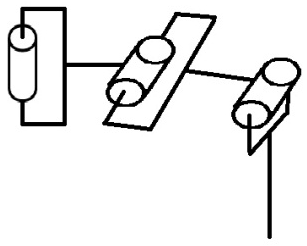
\includegraphics[width =0.8\textwidth]{figure_e}
	\caption{Three DoF solution}
	\label{figure_e}
\end{figure}

The design consists of links connected through knee joints. The walking motion is accomplished by controlling the angle of the links to position the feet. There are a number of different ways in which the joints can be actuated. Options include mounting the motor at the joint itself, or using a pulley and belt \ref{figure_f} or lead screw \ref{figure_g} to set the angle of the knee using an actuator mounted near the base of the leg.

\begin{figure}[H]
	\centering
	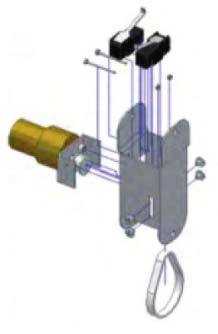
\includegraphics{figure_f}
	\caption{Pinion-belt arrangement}
	\label{figure_f}
\end{figure}

\begin{figure}[H]
	\centering
	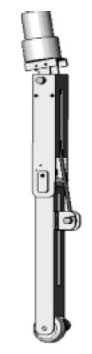
\includegraphics{figure_g}
	\caption{Lead screw leg}
	\label{figure_g}
\end{figure}

The major drawback of last design is the necessity to actuate remote joints. On the other hand, latching the actuator at the knee joint adds various dynamic effects to the leg which have to be compensated by the controller. This adds complexity to the control algorithms needed to move the leg.\\
It also requires more powerful motors at the hip joint to move the added mass of the leg. Remote actuation, in which the actuators are located at the base of the leg, eliminates some of these problems, at the cost of increasing the complexity of the mechanism. The coupling of the motion of the end effector relative to the actuators is another undesirable characteristic of this leg design.  Another potential leg design is modeled according to a typical mammalian leg with a four-bar linkage structure. The major drawback of this design is that the motions are highly coupled and the effective workspace is somewhat limited. Moreover, the entire weight of the robot is supported by the hip joint and they necessitate a powerful and expensive motor.

\section{Walking Gaits}
A gait is a sequence of leg motions coordinated with a sequence of body motions for moving the overall body of the robot in the desired direction and for orientation from one place to another. A gait is described as periodic when similar states of the same leg during successive strokes occur at the same interval for all legs. Periodic gaits are suitable for smooth terrain and they have been studied by several investigators. Figure 9 shows the scheme of some periodical hexapod gaits; white color indicates that the foot is in ground contact and the black color otherwise. Figure 9a reports the hexapod legs’ description.

\subsection{Tripod gait}
Tripod gait is a regular, periodic gait where the anterior and posterior legs on one side lift in time with the contralateral middle leg, forming alternating tripods. Thus, it is based on two groups of legs. During each step the first group of the legs is lifted and is rotated forward and is laid upon on the ground. Then the other group is lifted. Now both groups are moving, the first group backward, the second group forward and finally the second group is laid on the ground. It is obvious that both groups perform the same movement, but they are shifted by half a period. Tripod gait is very fast, but also very unstable. That is because at one moment half of the whole weight of the robot is only on one leg, which can lead to slip or even to fall. This is a gait suitable for high speed walking over relatively flat ground.

\subsection{Wave Gait}
Another gait is wave, which is the most stable gait, but also the slowest. Wave gait consists of a sequential adjustment of legs forward and only when all the legs are set to the new positions, the step is completed. In each phase of step maximally one leg is lifted up, which leads to high stability of this gait.

\subsection{Ripple Gait}
Ripple gait is inspired by insects. Each leg performs the same move – up, forward, down, backward.

\begin{figure}[h]
	\centering
	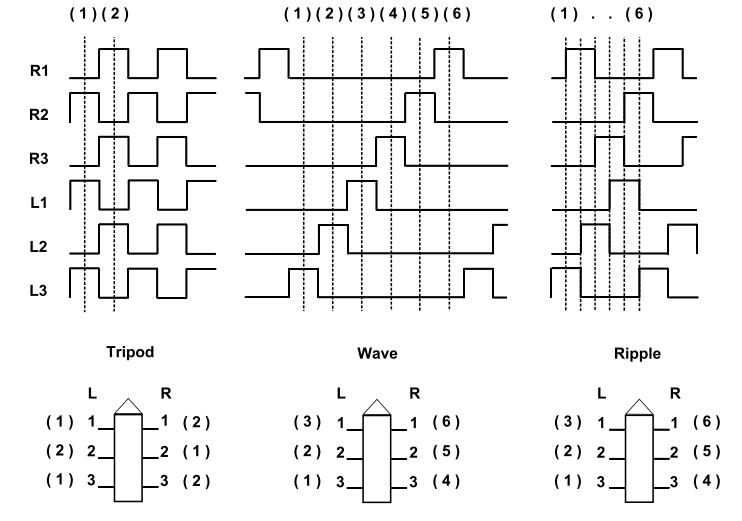
\includegraphics[width =0.8\textwidth]{figure_h}
	\caption{Gait diagram of hexapodal gaits}
	\label{figure h.png}
\end{figure}

\ref{figure h.png} shows the movement of each leg in time. A high value represents leg movement and low values means no movement. Tripod, wave and ripple gaits are shown in this figure. Tripod has two group of legs, all the legs in the same group move at once. In the wave gait only one leg is moving at any time. After all legs are set up to their new positions, step is completed. In the ripple gait all legs move the same way, but their moves are shifted. Leg moves partially overlap. In other words, the time when the first foot is lifted and begins to move forward, the second leg begins to lift up. In this way the robot cycles through all legs.

These are the most common gaits. Theoretical number of different gaits N can be calculated using equation: N = (2K - 1)!, where K is the number of the legs of the robot. Not all of them are usable for effective locomotion. For hexapod robot it is 11! = 39 916 800 possibilities of locomotion. The number is quite large, because this equation calculates all possible motions, like motion up and down, which of course doesn’t lead to an effective movement.

\section{Robot Kinematics}

\subsection{Robot body frame}
The origin of the robot base frame will be in the center of the body, structured with Z-axis pointing up, the X-axis positioning right and Y-axis pointing forwards with respect to the robot front side as depicted in \ref{Loc}.

\begin{figure}[h]
	\centering
	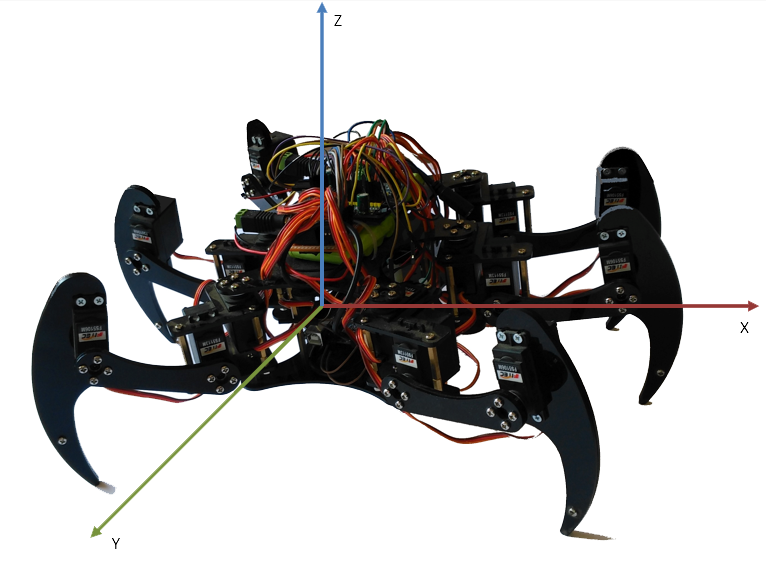
\includegraphics[width =0.8\textwidth]{Fig3}
	\caption{ Location of body frame relative to robot hardware.}
	\label{Loc}
\end{figure}

\subsection{Leg frames and notations}
The design of hexapod constitutes the kinematic configuration of a hexapod robot, with each leg acting as an independent serial manipulator with three degrees of freedom. Figure \ref{fig1} shows the actual prototype of our robot.

\begin{figure}[h]
	\centering
	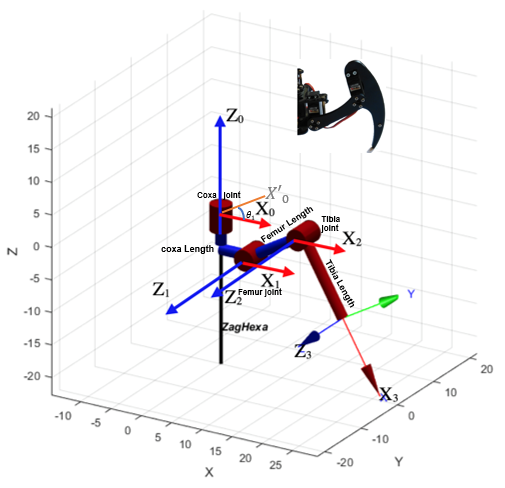
\includegraphics[width =.8\textwidth]{fream}
	\caption{  Final leg design (top right) and its notations, reference frames, joints and links.}
	\label{fream}
\end{figure}

The final leg design and its links and joints notations are given in \ref{fream}. The robot leg is made of links and joints as noted on \ref{leg}, different links of robot leg are called Femur, Tibia and Tarsus. As depicted in figure, the robot leg frame starts with link 0, which is the point where the leg is attached to the body, link 1, is Femur, link 2 is the Tibia and link 3 is Tarsus. The joints are located at the inner end of their respective link. Frames are attached to outer end of their respective links, this means that joint 2 rotates about the Z-axis of frame 1.

\begin{figure}[h]
	\centering
	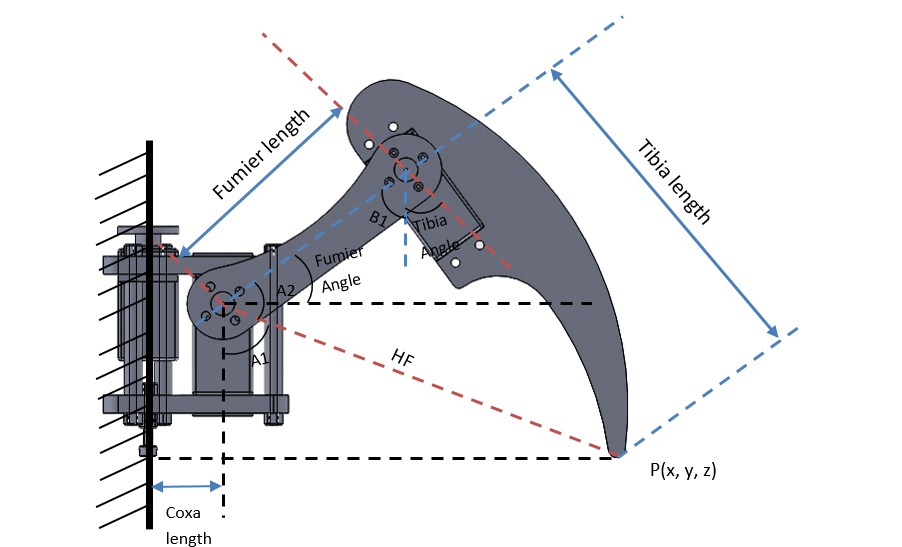
\includegraphics[width =.8\textwidth]{Fig7}
	\caption{  Final leg design (top right) and its notations, reference frames, joints and links.}
	\label{leg}
\end{figure}

\subsection{Robot Leg Parameters}
Following the well-known Denavit-Hartenberg (DH) notation, coordinate frames for the robot leg are assigned. The assigned frames are shown in \ref{leg}. In figure, the body {b} and the zeroth {0} reference frames are attached to the stationary robot body. Therefore, they can be both considered as inertial frames. The axes of the body frame are arranged to be in accord with the actual robot-body orientation. The DH link parameters based on \ref{leg} are given in Table II.\\

The resulting homogeneous transformation matrices between the body and the zeroth frame and between the sequential link frames are given in (1).  In the formulas, the variables represented by $a$ stand for the length of the $i^{th}$ link (namely, the length of the portion of the link between the origins of $(i-1) th and i^{th}$ reference frames). The variables represented by $\theta_{ij}$ mean the sum of the $i^{th}$ and $j^{th}$ joint angles $(\theta_{ij}=\theta_i+\theta_j)$. C and S are for cos(.) and sin(.) functions, respectively.  The exact values of these variables corresponding to ZagHexa robot are: 
$\psi = 45^\circ, a_1= 5cm, a_2= 9cm, a_3= 18cm$
\begin{center}
\begin{tabular}{|c||c|c|c|c|}
	\hline
	Joint & $\theta_i$ & $\alpha_i$ & $a_i$ & $d_i$ \\ \hline
	1&		$\theta_1$ & $\pi/2$	& $a_1$ & 0 \\ \hline
	2&		$A_2$ & 0			& $a_2$ & 0 \\ \hline
	3&		$B_1$ & 0			& $a_3$ & 0 \\ \hline
\end{tabular}
\end{center}

Homogeneous matrices are used in derivation of positional relations between the successive frames.  In (3) the leg tip point position with respect to the body frame is given. The rotation matrices between the frames are given in (2). These rotation matrices are used in vector equations, especially while deriving the dynamic equations.
\begin{center}

\[
H^{(b,0)}=
\begin{bmatrix}
0 & \cos(\psi) & \sin(\psi) & 0 \\
-1&		0	   & 		0 	& 0\\
0 & -\sin(\psi)& \cos(\psi) & 0 \\
0 &		0	   & 		0 	& 1
\end{bmatrix}
\]
\end{center}

\begin{equation}
H^{(K-1,K)} =
\begin{bmatrix}
\cos\theta_k &-\cos\alpha_k\sin\theta_k &\sin\alpha_k\sin\theta_k &a_k\cos\theta_k\\
\sin\theta_k &\cos\alpha_k\cos\theta_k &-\sin\alpha_k\cos\theta_k &a_k\sin\theta_k\\
0 &\sin\alpha_k &\cos\alpha_k &d_k \\ 
0 &0 &0 &1
\end{bmatrix}
\end{equation}

\begin{align*}
H^{(0,3)} = H^{(0,1)} H^{(1,2)} H^{(2,3)} H^{(b,3)}= H^{(b,0)} H^{(0,3)}
\end{align*}

\begin{center}
	
	\[
	C^{(b,0)}=
	\begin{bmatrix}
	0 & \cos(\psi) & \sin(\psi) \\
	-1&		0	   & 		0 	\\
	0 & -\sin(\psi)& \cos(\psi) \\

	\end{bmatrix}
	\]
\end{center}

\begin{equation}
C^{(K-1,K)} =
\begin{bmatrix}
\cos\theta_k &-\cos\alpha_k\sin\theta_k &\sin\alpha_k\sin\theta_k \\
\sin\theta_k &\cos\alpha_k\cos\theta_k &-\sin\alpha_k\cos\theta_k \\
0 &\sin\alpha_k &\cos\alpha_k \\ 
\end{bmatrix}
\end{equation}
\begin{equation}
P_e^{(K-1,K)} (\theta) =
\begin{bmatrix}
C\psi(a_1S\theta_1+a_2S\theta_1C\theta_2+a_3S\theta_1C\theta{23})+S\psi(a_2S\theta_2+a_3\theta_{23}) \\
-(a_1C\theta_1+a_2C\theta_1C\theta_2+a_3C\theta_1C\theta_{23})  \\
-S\psi(a_1S\theta_1+a_2S\theta_1C\theta_2+a_3S\theta_1C\theta{23})+C\psi(a_2S\theta_2+a_3\theta_{23}) \\
\end{bmatrix}
\end{equation}
To derive the dynamic equations, first the inertia matrices of the links should be determined. Since the $k^{th}$ reference frame is stationary with respect to the $k^{th}$ link, the inertia tensor of the $k^{th}$ link around its center of mass appears to be a constant matrix with respect to the $k^{th}$ reference frame, as in (4). The values used in these formulations belong to the Hexapod robot. The resulting matrices for each link are in the form of (5).
\begin{equation}
\{J_K\}^{(K)} = J_K^{(K)} = J_K
\end{equation}
\begin{equation}
J_K = \begin{bmatrix}
J_{K1} & 0      & 0 \\
0      & J_{K2} & 0 	\\
0      & 0      & J_{K3} 
\end{bmatrix}
\end{equation}


\subsection{Inverse kinematics}
The forward kinematics (FK) is a simple equation used to calculate the position of the end effectors for the leg in the robot base frame, by injecting values of each joint angle. But the reverse operation, namely inverse kinematics (IK), is more complex. IK is employed to find all the joint angles given the position of the end effectors. In general, solving the IK equations can be a bit of a challenge. Some positions cannot be reached at all, as the physical system is unable to get there, and some end effectors positions can have more than one solution, and not all of them are desirable.

We solve the IK problem for each leg separately, as this makes it possible to solve it geometrically, by setting up some constrains. The first constraint for solving the IK equations due the fact that all robot joints allow rotation about one axis only. The second constraint is that the Femur, Tibia joints always rotate on parallel axes. The third set of constraints arises from the physical limitations for each joint, giving us some angular interval for each joint in which the servos can actually rotate the link. In \ref{leg}, the angles of movement are shown.
First, the coxa angle can be found directly by knowing the end effectors position then simply using $atan2(y,x)$ to calculate it. Equations (6) through (14) are used to find the individual joint angles.
\begin{figure}[h]
	\centering
	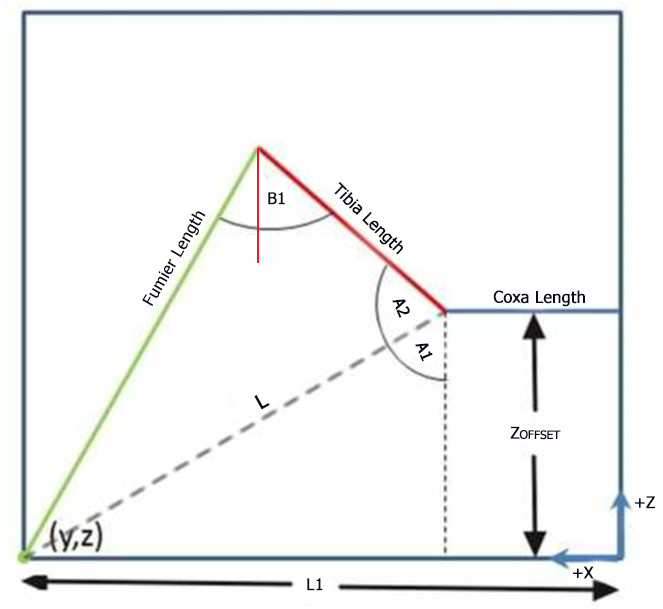
\includegraphics[width =.6\textwidth]{Fig8.png}
	\caption{ Illustration of the 2D triangle with vertices in the coxa, the femur, and tibia link from origin.}
	\label{fig8}
\end{figure}

\begin{align}
    \frac{x}{y} & =\tan (y)\to \gamma =\tan ^{-1}\frac{x}{y} \\
    L              & = \sqrt{Z_{offset}^{2}+(L_{1}+\cos A)^{2}}\\
    a_{L}        & = \cos ^{-1}(\frac{Z_{offset}}{L})\\
    Tibia^{2}  & =Femar^{2}+L^{2}-2(Femar)(L)\cos \alpha _{2} \\
    \alpha _{2} & =\cos^{-1}(\frac{Tibia^{2}-Femar^{2}-L^{2}}{-2(Femar)(L)}) \\
    \alpha      & =\alpha _{1}+\alpha _{2}\\
    \alpha      & = \cos ^{-1}(\frac{Z_{offset}}{L})+\cos ^{-1}(\frac{Tibia^{2}-Femar^{2}-L^{2}}{-2(Femar)(L)}) \\
    \beta        & = \cos^{-1}(\frac{L^{2}-Femar^{2}-Tibia^{2}}{-2(Femar)(Tibia)}
\end{align}